\section{Reichweitenbestimmung}
%kurz das ziel dieses versuchsteiles ansprechen, damit keine zwei �berschriften direkt �bereinander stehen!
%bei schwierigeren versuchen kann auch der theoretische hintergrund erl�utert werden. (mit formeln, herleitungen und erkl�rungen)
Es soll die Reichweite von $\alpha$-Strahlung bei Normaldruck untersucht werden.

\subsection{Versuchsdurchf�hrung}
Es werden keine Metallfolien oder Kollimationsspalte verwendet. Der Schwenkarm wird auf 0$^\circ$ eingestellt. Da der Abstand zwischen dem $^{241}$Am-Pr�parat und der Quelle nicht ver�nderbar ist (5,0 $\pm$ 0,5 cm), kann die Abstandsabh�ngigkeit nicht direkt bestimmt werden. Stattdessen wird die Z�hlrate in Abh�ngigkeit des Luftdrucks aufgenommen. Da die Reichweite linear mit Anzahl der St��e mit den Luftmolek�len abh�ngt, h�ngt die Reichweite unter Annahme des idealen Gassesetztes auch linear von Druck ab. Daraus l�sst sich f�r die Reichweite unter Normaldruck Gleichung \ref{eqn:reich_normal} folgern.

\begin{align}
\label{eqn:reich_normal}
x_{Messung} = x_{Normal} \frac{p_{Messung}}{p_{Normal}} 
\end{align}

Der Fehler ergibt sich nach Gleichung 

\begin{align}
\label{eqn:delta_reich_normal}
\Delta x_{Messung} = x_{Normal} \frac{\Delta p_{Messung}}{p_{Normal}} 
\end{align}

Der Druck wird solange erh�ht, bis die Countrate auf 0 abf�llt. Da der Abfall der Z�hlrate jedoch gau�verschmiert ist, muss der Nullpunkt mit einer logistischen Regression bestimmt werden. F�r die logistische Regression wird Gleichung \ref{eqn:logi} verwendet. Mit dem Zusammenhang, aus Gleichung \ref{eqn:reich_normal} kann die Reichweite von $\alpha$-Strahlung in Luft bestimmt werden.

\begin{align}
\label{eqn:logi}
f(x) = B + \frac{A-B}{1 + \left( \frac{x}{D} \right)^C}
\end{align}

Die Messwerte mit dem Fit sind in Abb. \ref{fig:reichweite} zu sehen, f�r den Fit ergeben sich die Werte in Tabelle \ref{tab:fit_logi}.


\begin{figure}[H]
	\centering
  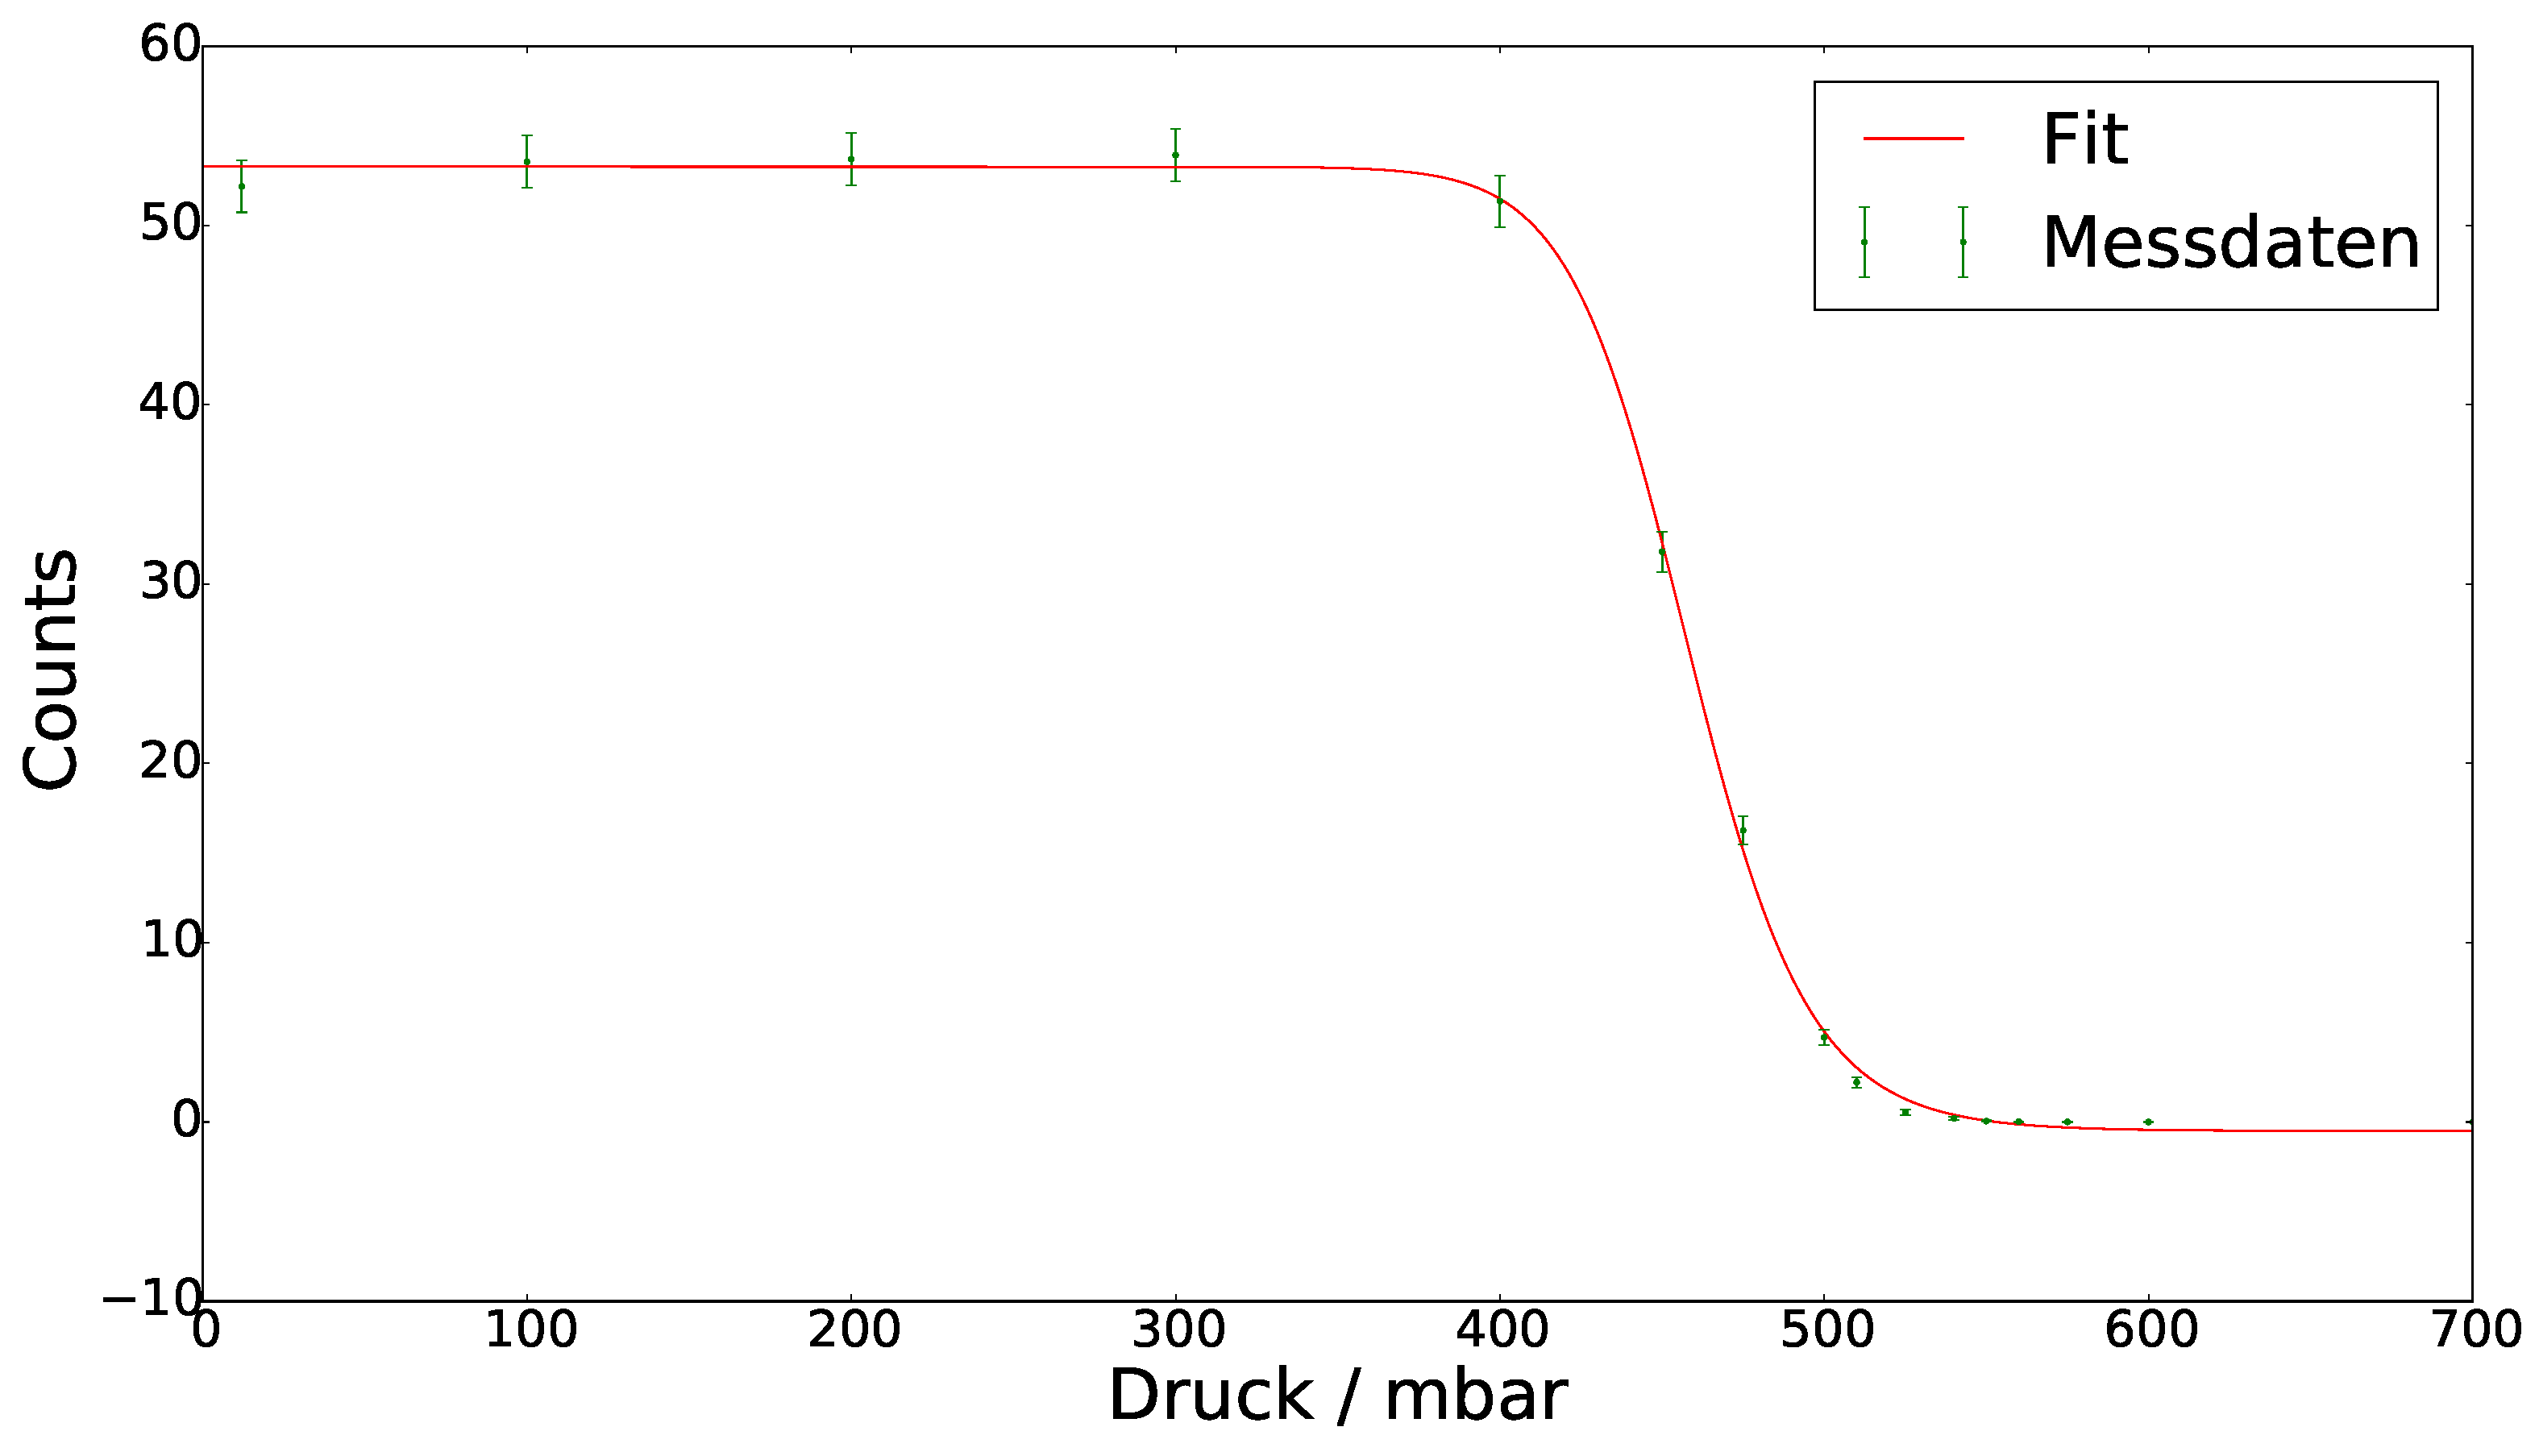
\includegraphics[scale=0.33]{reichweite.pdf}
	\caption{Es sind die Messdaten aus der Streuung von $\alpha$-Strahlung an Gold, bei unterschiedlichem Druck zu sehen. Die Messdaten wurden mit  Gleichung \ref{eqn:logi} gefittet, dabei ergab sich ein $\chi_{red}^2$ von 0,45.}
	\label{fig:reichweite}
\end{figure}

\begin{table}
\centering
\caption{Parameter des Fits zur Bestimmung der Reichweite von $\alpha$-Strahlung in Luft. F�r den Fit wurde Gleichung \ref{eqn:logi} verwendet.}
\label{tab:fit_logi}
\begin{tabular}{|c|c|}
\hline Parameter & Wert \\ 
\hline A & 25,0 $\pm$ 1,0 \\ 
\hline B & 458,2 $\pm$ 0,8 \\ 
\hline C & 53,3 $\pm$ 0,3 \\ 
\hline D & -0,5 $\pm$ 0,3 \\ 
\hline $\chi_{red}^2$ & 0,45 \\ 
\hline 
\end{tabular} 
\end{table}

Die Daten werden gut durch die logistische Regression beschrieben, aus den Fitparametern kann mit Gleichung \ref{eqn:p_0} der Druck bestimmt werden, bei dem die Z�hlrate auf 0 abgefallen ist.

\begin{align}
\label{eqn:p_0}
p_0 = D \sqrt[C]{\frac{A}{B}}
\end{align}



Mit den bestimmten Parametern aus Tabelle \ref{tab:fit_logi} ergibt sich ein Druck von 504 $\pm$ 34 mbar. Bei einem Normaldruck von p$_{normal}$ = 1013,25 mbar und einem Abstand von x$_0$ = 5 $\pm$ 0,5 cm kann mit Gleichung \ref{eqn:reich_normal} die Reichweite der $\alpha$-Strahlung in Luft bestimmt werden. Es ergibt sich eine Reichweite von 2,5 $\pm$ 0,3 cm.  Dieser Wert muss jedoch korrigiert werden, da durch die 3$\mu$m dicke Goldfolie die Energie der $\alpha$-Strahlung von 5,5 MeV auf 4,5 MeV abgeschw�cht wird. Es ergibt sich damit ein Korrekturfaktor nach Gleichung \ref{eqn:korrekur} welcher multiplikativ in Gleichung \ref{eqn:reich_normal} eingeht. Damit ergibt sich ein korregierter Wert von 3,04 $\pm$ 0,37. Erwartet wurde ein Wert von 2,96 cm, dieser Wert wurde mit der empirischen Reichweite nach Geiger bestimmt (siehe \cite{wiki_geiger}). Der Korrigierte Wert weicht um 2,7\% ab, was ein gutes Ergebnis ist, wobei der Erwartete Wert innerhalb der Fehler des gemessenen liegt.



\begin{align}
\label{eqn:korrekur}
f_{korrektur} = \frac{5,5 MeV}{4,5 MeV}
\end{align}
